\documentclass[notes]{beamer}       		% compila sia i frame che le note
%\documentclass{beamer}              				% compila solo i frame
%\documentclass[notes=only]{beamer}  	% compila solo le note

% ita language and encoding
\usepackage[utf8]{inputenc}
%\usepackage[italian]{babel}

% formattazione
\usepackage{ragged2e} 							% pacchetto che contiene il comando \justifying
%\apptocmd{\frame}{}{\justifying}{}  	% --> applica la giustificazione a tutti i frame del documento
%\justifying											% --> applica la giustificazione a tutto il documento

% graphics style
\usepackage{graphicx}
\usepackage{xcolor}
\usepackage{shadowtext}

%tabelle
\usepackage{tabularx}
\usepackage{multirow}
\usepackage{booktabs} % aggiunge: \toprule , \midrule e \bottomrule ; stile tabella

%image paths
\graphicspath{	
	{./Images/}
}

% impostazioni base delle slide - tema, colori, caratteri, ... (deic.uab.es/~iblanes/beamer_gallery/)
\mode<presentation>
{
	%\usetheme{CambridgeUS}      	% or try Darmstadt, Madrid, Warsaw, ...
  	\usecolortheme{orchid} 				% for the color box (or try rose ...)
	\usefonttheme{structurebold} 	% or try structureitalicserif, structuresmallcapsserif
}



%% ---------------------------------------------------------------------------------------------------------
% %	CREAZIONE TEMA 

%%    Impostazione dei colori - COLORTHEME 
% (modifica di "beamercolorthemebeaver.sty" in "MiKTeX 2.9/tex/latex/beamer/themes/color" )
\definecolor{darkblue}{RGB}{52,57,176}

\setbeamercolor{section in toc}{fg=black,bg=white}
\setbeamercolor{alerted text}{fg=darkblue!80!gray}
\setbeamercolor*{palette primary}{fg=darkblue!60!black,bg=gray!30!white}
\setbeamercolor*{palette secondary}{fg=darkblue!70!black,bg=gray!15!white}
\setbeamercolor*{palette tertiary}{bg=darkblue!80!black,fg=gray!10!white}
\setbeamercolor*{palette quaternary}{fg=darkblue,bg=gray!5!white}

\setbeamercolor*{sidebar}{fg=darkblue,bg=gray!15!white}

\setbeamercolor*{palette sidebar primary}{fg=darkblue!10!black}
\setbeamercolor*{palette sidebar secondary}{fg=white}
\setbeamercolor*{palette sidebar tertiary}{fg=darkblue!50!black}
\setbeamercolor*{palette sidebar quaternary}{fg=gray!10!white}

%\setbeamercolor*{titlelike}{parent=palette primary}
\setbeamercolor{titlelike}{parent=palette primary,fg=darkblue}
\setbeamercolor{frametitle}{bg=gray!10!white}
\setbeamercolor{frametitle right}{bg=gray!60!white}

\setbeamercolor*{separation line}{}
\setbeamercolor*{fine separation line}{}


%%     Impostazione dei blocchi - INNERTHEME 
% (modifica di "beamerinnerthemerounded.sty" in "MiKTeX 2.9/tex/latex/beamer/themes/inner" )
%\setbeamertemplate{blocks}[rounded]
\setbeamertemplate{items}[ball]
%\setbeamertemplate{sections/subsections in toc}[ball]
%\setbeamertemplate{title page}[default][colsep=-4bp,rounded=true]
%\setbeamertemplate{part page}[default][colsep=-4bp,rounded=true]


%	%    Impostazione delle intestazioni - OUTERTHEME
% (modifica di "beamerouterthemeinfolines.sty" in "MiKTeX 2.9/tex/latex/beamer/themes/outer" )
\setbeamercolor{institute in head/foot}{parent=palette secondary}
\setbeamercolor{subject in head/foot}{parent=palette tertiary}
\setbeamercolor{title in head/foot}{parent=palette primary}
\setbeamertemplate{footline}
{ 
	\leavevmode%
	\hbox{%
  		% "ht" è lo spazio sopra il carattere partendo dalla base del carattere, "dp"  è lo spazio sotto il carattere partendo sempre dalla base del carattere
  		\begin{beamercolorbox}[wd=.333333\paperwidth,ht=2.5ex,dp=1ex,left,leftskip=4ex]{author in head/foot}%
   			\usebeamerfont{author in head/foot}\insertshortauthor
  		\end{beamercolorbox}%
  		\begin{beamercolorbox}[wd=.333333\paperwidth,ht=2.5ex,dp=1ex,center]{institute in head/foot}%
    		\usebeamerfont{title in head/foot}\insertshortinstitute
 		 \end{beamercolorbox}%
 		 \begin{beamercolorbox}[wd=.333333\paperwidth,ht=2.5ex,dp=1ex,right,rightskip=4ex]{date in head/foot}%
 		 	\usebeamerfont{date in head/foot}\insertshortdate{}\hspace*{2em}\insertframenumber{} / \inserttotalframenumber
 		 \end{beamercolorbox}
 		 }%
 	\vskip0pt%
}
\makeatletter
\setbeamertemplate{headline}
{
  \leavevmode%
  \hbox{%
  \begin{beamercolorbox}[wd=.5\paperwidth,ht=2.8ex,dp=1.35ex,left]{subject in head/foot}	
    \usebeamerfont{section in head/foot}\hspace*{4ex}Complements of Condensed Matter Physics			% --> N.B. Qui c'è l'unica scritta che non usa nessun template tipo \title o \institute
  \end{beamercolorbox}%
  \begin{beamercolorbox}[wd=.5\paperwidth,ht=2.8ex,dp=1.35ex,right]{title in head/foot}%
    \usebeamerfont{subsection in head/foot}\insertshorttitle\hspace*{4ex}
  \end{beamercolorbox}}%
  \vskip0pt%
}
\makeatother

%%    FINE IMPOSTAZIONI TEMA
%% ---------------------------------------------------------------------------------------------------------



% settagio dati principali del file - titolo, autore, ...
\title[Selected concepts of Molecular Dynamics Simulation]{Molecular Dynamics Simulation}
\subtitle{A brief introduction of selected concepts}
\author{Daniele Di Bari}
\institute{University of Perugia}
\date{5th March 2018}
\subject{Complements of Condensed Matter Physics}

% By default the beamer class adds navigation buttons in the bottom right corner. To remove them one can place
\beamertemplatenavigationsymbolsempty

% settaggio prima slide
\setbeamertemplate{title page}
{
	\shadowcolor{white!30!black}
	\vspace{1.5cm}	   
    
    	
    \begin{colorbox}{darkblue}{ \parbox{0.8\paperwidth}{
    	\shadowtext{\textcolor{white}{\textbf{\footnotesize{ }}}}
    	
    	\vspace{0.2cm}  	
    	
    	\shadowtext{\textcolor{white}{\textbf{\LARGE \inserttitle}}}\par
    	
    	\vspace{0.1cm}  
    	
    	\shadowtext{\textcolor{white}{\emph{\large \insertsubtitle}}}\par
    	
    	\vspace{0.2cm}  
    	}}
    \end{colorbox} 
   	
   	\vspace{2.5cm}
	
	\titlepagetext{lightgray}{The general particle physics}\\
	\titlepagetext{lightgray}{experiment in space, on board}\\
	\titlepagetext{gray}{the International Space Station}\\
	\titlepagetext{gray}{since 19th May 2011.}		
}
				
% colors
\definecolor{itemred}{RGB}{163,0,0}
\definecolor{itemblue}{RGB}{52,57,176}
\definecolor{notegrey}{RGB}{90,90,90}
\definecolor{titlebgd_grey}{RGB}{242,242,242}
\definecolor{titleframe_red}{RGB}{204,0,0}

% COMANDI
% Formato testo generico in titolpage
\newcommand\titlepagetext[2]{\textcolor{#1}{\footnotesize{\textit{{#2}}}}}
\newcommand\colortextbf[2]{\textcolor{#1}{\textbf{#2}}}
\newcommand\bluetextbf[1]{\textcolor{itemblue}{\textbf{#1}}}
\newcommand\bluetextit[1]{\textcolor{itemblue}{\textit{#1}}}
\newcommand\textitem[2]{\textcolor{itemblue}{\textbf{#1} (\textit{#2})}}

% Testo giustificato
\newenvironment<>{justify}{\justifying{}}

\begin{document}
	% impostare una foto come sfondo del frame: 
	%  \usebackgroundtemplate{\includegraphics[height=\paperheight,keepaspectratio]{on_ISS-08_cutMIDDLEUP-3088.jpg}}	
	% 	possibili impostazioni per l'img: width=\paperwidth  --  height=\paperheight  --  keepaspectratio

\begin{frame}\pdfbookmark[2]{Title}{Title}
	\titlepage
\end{frame}

\note{ 
\footnotesize{
There are a range of techniques of a quasi-experimental character, referred to collectively as computer simulation, the importance of which in the development of liquid state theory can hardly be overstated.
The usefulness of computer simulation relies on the fact that a sample containing a few hundred or few thousand particles is in many cases sufficiently large to simulate the behaviour of a macroscopic system. 
There are two classic approaches: molecular dynamics and Monte Carlo. 
Molecular dynamics has the advantage of allowing the study of time-dependent processes, but for the calculation of static properties a Monte Carlo method may be more efficient. 
We will focus on the first.
}
}

\usebackgroundtemplate{}

%\begin{frame}[allowframebreaks]\pdfbookmark[2]{Contents}{Contents}
%\frametitle{Table of Contents}
%\tableofcontents
%\end{frame}

\begin{frame}<presentation:0>[noframenumbering]
frame rimosso dalla presentazione
\end{frame}

\section{Introduction}
\begin{frame}
	\setbeamertemplate{background}{white}
	\frametitle{Introduction}
	\framesubtitle{The problem of describing complex system}
	\justifying
	
	Few systems in statistical mechanics are exactly soluble, the majority require approximations, but when their complexity increases 
	it becomes difficult even to construct an approximate theory in a reasonable way. 
	
	\vspace*{0.4cm}
	
	\textbf{The more complex and realistic is a system, the more difficult and interesting it becomes to describe it.} 
	
	\vspace*{0.4cm}
	
	In this case, an increase in the complexity raises the necessity of having exact results available, both to test existing 
	approximation methods and to point the way towards new approaches. 	
	
\end{frame}


\begin{frame}
	\frametitle{Introduction}
	\framesubtitle{Why to use Computer Simulation?}
	\justifying
	Computer simulations allow to calculate the essentially exact results for a given model without having to rely on approximate theories. 
	
	\begin{itemize}\justifying
		\item[$\blacktriangleright$] \textbf{TEST THE MODELS:} comparing the results of the simulation with those of a real experiment. 
		If there is disagreement, the model is inadequate - it is necessary to improve on the estimate of the intermolecular interactions.
		\item[$\blacktriangleright$] \textbf{TEST THE THEORIES:} comparing the results of the simulation with the predictions of an 
		approximate analytical theory applied to the same mode. If there is disagreement, the theory is flawed.\footnotemark[1] 
	\end{itemize}	
	
	\footnotetext[1]{The computer simulation plays the role of the experiment designed to test the theory. 
	This method of screening theories before we apply them to the real world is called a computer experiment.}
\end{frame}

\note{

}


\begin{frame}
	\frametitle{Introduction}
	\framesubtitle{the principal steps of a molecular simulation}
	\justifying
	
	The most common application of computer simulations is to predict the properties of materials (also of materials that have not yet been made) because they are like a ``virtual laboratory'' and they have the advantage that many such ``experiments'' can be easily set up and carried out in succession by simply varying the control parameters.

Extreme conditions, such as high $T$ and $p$, can be created in a simple and considerably safer manner. 

The obvious downside is that the results are only as good as the numerical model. In addition, the results can be artificially biased if the molecular dynamics calculation is unable to sample an adequate number of microstates over the time it is allowed to run.
	
\end{frame}

\begin{frame}
	\frametitle{Introduction}
	\framesubtitle{the principal steps of a molecular simulation}
	\justifying

Computer simulation provides a direct route from the microscopic details of a system (...) to macroscopic properties of experimental interest (...). As well as being of academic interest, this type of information is technologically useful. It may be difficult or impossible, while a computer simulation of the material in, say, a shock wave, a high-temperature plasma, nuclear reactor, or a planetary core, would be perfectly feasible. 

Quite subtle details of molecular motion and structure, for example in heterogeneous catalysis, fast ion conduction, or enzyme action, are difficult to probe experimentally, but can be extracted readily from a computer simulation.

Finally, while the speed of molecular events is itself an experimental difficulty, it presents no hindrance to the simulator. A wide range of physical phenomena, from molecular to the galactic, may studied using some form of computer simulation.
	
\end{frame}


\begin{frame}
	\frametitle{Introduction}
	\framesubtitle{the principal steps of a molecular simulation}
	\justifying
	
	\vspace*{0.1cm}

	A molecular-scale computer simulation consists of 3 principal steps:
	
	\begin{enumerate}\justifying
		\item Construction of a model
		\item Calculation of molecular trajectories
		\item Analysis of those trajectories to obtain property values
	\end{enumerate}
	
	\vspace*{0.2cm}

	The second step constitutes the \textbf{main feature} of the simulation. In a way that molecular positions $\bold{r}^N$ are computed 
	in this step, thus it is possible to discriminate among the different simulation methods.
	
	\vspace*{0.2cm}
	
	\begin{center}
		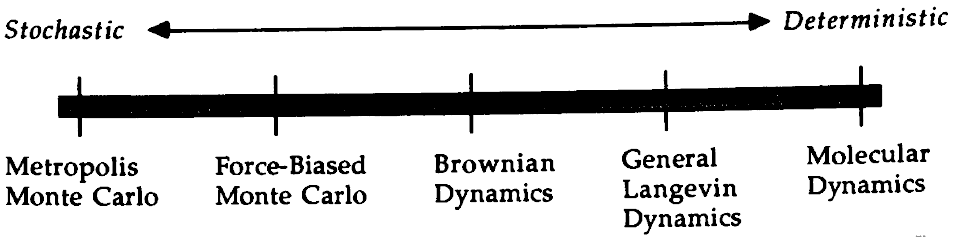
\includegraphics[width=0.7\textwidth]{different_tipes_of_CS.PNG}
	\end{center}
	
\end{frame}

\note{
In \textbf{molecular dynamics} the positions are obtained by numerically solving differential equations of motion and, hence, the positions are connected in time - the positions reveal dynamics of individual molecules as in a motion picture. 

\vspace*{0.2cm}

In other simulation methods the molecular positions are not temporally related. For instance, in \textbf{Monte Carlo} simulations the positions are generated stochastically such that a molecular configuration $\bold{r}^N$ depends only on the previous configuration. When the outcome of a random event in a sequence depends only on the outcome of the immediately previous event, the sequence is called a Markov chain.

\vspace*{0.2cm}

However in \textbf{other simulation methods}, the positions are computed from hybrid schemes that use some stochastic features, as in Monte Carlo, and some deterministic features, like in Molecular Dynamics.
}


\begin{frame}
	\frametitle{Introduction}
	\framesubtitle{What is a MD Simulation?}
	\justifying
	Molecular Dynamics simulation is a technique for computing the equilibrium and transport properties of a classical many-body system. 
	In this context, the word classical means that the nuclear motion of the constituent particles obeys the laws of classical mechanics. 
	This is an excellent approximation for a wide range of materials.
	Only when we consider the translational or rotational motion of light atoms or molecules (He, $\text{H}_2$, $\text{D}_2$) 
	or vibrational motion with a frequency $\nu$ such that $h \nu < k_B T$ should we worry about quantum effects.
\end{frame}

\begin{frame}
	\frametitle{Introduction}
	\framesubtitle{What is a MD Simulation?}
	\justifying
	Molecular Dynamics simulation is a technique for computing the equilibrium and transport properties of a classical many-body system. 
	In this context, the word classical means that the nuclear motion of the constituent particles obeys the laws of classical mechanics. 
	This is an excellent approximation for a wide range of materials.
	Only when we consider the translational or rotational motion of light atoms or molecules (He, $\text{H}_2$, $\text{D}_2$) 
	or vibrational motion with a frequency $\nu$ such that $h \nu < k_B T$ should we worry about quantum effects.
\end{frame}
\note{
\footnotesize{
We will assume that the motion of the nuclei can be described by Newton's law. This approximation breaks down clearly for very light atoms (H, De, He) and for all vibrational motions whose characteristic frequency, translated in energy, is comparable or larger than the thermal energy $k_{B} T$.
Performing numerical simulations, we sample the system phase-space and hence we have access to positions rN and momenta pN of all atoms in the system. From this information the microscopic value of all observables which are function of (rN,pN) can be evaluated and, eventually, averaged over time or phase-space.
Numerical simulations can be considered as a tool for performing numerical experiments. In this respect, simulations can be used for different applications: 
reproduce an existing experimental result, to complement the macroscopic information with the atomistic level provided by the simulation;
to produce a numerical prediction of a gedanken experiment;
for checking theoretical approximations based on model systems.
}
}

\section{Technical Requirements}
\subsection{from Physics Goals}
\begin{frame}
    \frametitle{Technical Requirements}
    \framesubtitle{from Physics Goals}
    \justifying
    
	Physical goals involve \textbf{technical requirements for the AMS detector}:
	
	\begin{itemize}\justifying
		\item	\bluetextbf{Dark Matter $\Rightarrow$}
					to get $e^+/p$ rejection of $\sim10^{-6}$ for the measurement of the positron fraction.
		\item	\bluetextbf{Matter/Antimatter Asymmetry $\Rightarrow$}
					to reach a sensitivity in the search for anti-matter nuclei of $10^{-10}$ (ratio of anti-helium nuclei to helium nuclei).
		\item	\bluetextbf{Cosmic Ray Physics $\Rightarrow$}
					to measure the composition and spectra of charged particles with an accuracy of 1\%.
	\end{itemize}
	
	Moreover, \bluetextbf{for each of these ones}, it is very important to extend, as far as possible, the energy range of the 
	measurements.
	
	For AMS, the required energy range is from 0.5 to $\sim$ 2000 $GeV$.

	%\footnotesize{\underline{\textbf{Note}} These requirements represent a considerable sensitivity improvement compared to the previous space-borne experiments.}

\end{frame}

\note{
	In a conventional molecular dynamics simulation of a bulk fluid a system of N particles is allocated a set of initial coordinates within a cell of fixed volume, most commonly a cube. A set of velocities is also assigned, usually drawn from a Maxwell distribution appropriate to the temperature of interest and selected in such a way that the net linear momentum of the system is zero. The subsequent calculation tracks the motion of the particles through space by integration of the classical equations of motion. Equilibrium properties are obtained as time averages over the dynamical history of the system in the manner outlined in Section 2.2 and correspond to averages over a microcanonical ensemble. In modern work N is typically of order 103 or 104, though much larger systems have occasionally been studied. To minimise surface effects, and thereby simulate more closely the behaviour expected of a macroscopic system, it is customary to use a periodic boundary condition.
}

\begin{frame}
	\frametitle{Technical Requirements}
    \framesubtitle{from Physics Goals}	
    
    \begin{block}{The technical challenge of AMS-02}
		\justifying
		The illustrated requirements represent a considerable sensitivity improvement compared to the previous space-borne 
		experiments.
	\end{block}
   	
   	\vspace{0.25cm}
	\small{\bluetextbf{NOTE}}
	\vspace{-0.2cm}
    \begin{itemize}
    	\item[\footnotesize{$\blacktriangleright$}] 
    		\footnotesize{\justifying
    		There is a strong demand for precision measurements of CRs in the energy region from 10 to 1000 
    		$GeV$ as the measurements of positron fraction, i.e.  $e^+ / (e^+ + e^-)$, by AMS-01, HEAT, PAMELA and FERMI 
    		indicate a large deviation of this ratio from the production of $e^+$ and $e^-$ predicted by a model that includes only 
    		ordinary CR collisions.
    		
    		These available measurements are both at too low an energy and of too limited statistics to shed the light on the origin of 
    		this significant excess.
    		
    		AMS-02 is expected to provide definitive answers concerning the nature of this deviation.}
   	\end{itemize}  
   	 
%
%%	\vspace{0.25cm}
%	There is a strong demand for precision measurements of cosmic rays in the energy region from 10 to 1000 GeV as the 
%	measurements of e+/(e+ + e-) by AMS-01, HEAT, PAMELA and FERMI indicate a large deviation of this ratio from the 
%	production of e+ and e- predicted by a model that includes only ordinary cosmic ray collisions. 
%	
%	These available measurements are both at too low an energy and of too limited statistics to shed the light on the origin of this 
%	significant excess. 
%	
%	AMS-02 is	expected to provide definitive answers concerning the nature of this deviation.
\end{frame}

%\begin{frame}
%	\frametitle{Technical Requirements}
%    \framesubtitle{From Physics Goals}
%	\begin{columns}
%		\begin{column}{0.5\textwidth}
%			\begin{center}
%				\includegraphics[width=0.95\columnwidth]{Schem_Requirements-DM.png}
%			\end{center}
%		\end{column}
%
%		\begin{column}{0.5\textwidth}
%			\begin{center}
%				\includegraphics[width=0.95\columnwidth]{Schem_Requirements-Antimatter.png}
%			\end{center}
%		\end{column}
%	\end{columns}
%\end{frame}

\begin{frame}[label=AMS-apparatus_img]
	\frametitle{Technical Requirement}
	\framesubtitle{general structure of the AMS apparatus}
	\begin{center}
		\vspace{-0.15cm}
		%\hspace{-0.35cm}\includegraphics[height=0.7\paperheight]{Schem_structure_of_AMS.png}

		\vspace{-0.35cm}

		\hspace{0.25cm}\hyperlink{AMS-apparatus_list}{\textbf{\beamerbutton{link to AMS apparatus list}}}
	\end{center}
	%\vspace{-0.25cm}
\end{frame}

\end{document}
